% !TEX encoding = UTF-8 Unicode
\chapter{Grundlagen zu auftragsbezogenen Instandhaltungsprozessen}\label{Instandhaltung}
\markboth{2 Grundlegende Begriffe}{}
\setcounter{footnote}{4}  %um durchgehende Fußnotennummerierung zu haben, hier die Anzahl der bisherigen Fußnoten eintragen

\section{Einordnung in die Produktionswirtschaft und Begriffsbestimmung}

Unter Instandhaltungsprozessen (engl. maintenance-repair-and\-overhaul; Abk. MRO)) wird in dieser Arbeit ein nachgelagerter Prozess eines erweiterten Leistungsprogramms eines Unternehmens verstanden und kann damit als Teilsystem angesehen werden, welches den gesamten Wertschöpfungsprozess verlängert. Es handelt sich nicht um die interne oder beauftragte Instandhaltung von u. a. Anlagen und technischen Systemen, sondern versteht eine Leistung eines Unternehmens. Im weiteren Verlauf dieser Arbeit ist unter Instandhaltung ein Prozess gemeint, der als (zusätzliche) Dienstleistung eines Unternehmens auf Basis einer Auftragsfertigung angeboten wird. D. h. das Unternehmen nimmt Kundenaufträge zur Instandsetzung von Produkten an und erzielt durch diese Leistung einen auftragsabhängigen Ertrag. Bei der auftragsbezogenen Instandhaltungsprozessen handelt es sich folglich um eine Produktion einer Leistung und kann damit der betriebswirtschaftlichen Betrachtung der Produktionswirtschaft zugeordnet werden.

Bei dem Begriff der Produktionswirtschaft handelt sich um ein Teilgebiet der Betriebswirtschaftslehre.\footnote{Neben der Teilgebiete Finanzwirtschaft, Marketing, Unternehmensführung, Unternehmensrechnung etc., vgl. dazu \cite{Dyckhoff2010}, S. 3.} In der Produktionswirtschaft wird der Fokus auf die Produktion von Leistung gelegt.\footnote{Vgl. \cite{Dyckhoff2010}, S. 3} Bei diesem ökonomischen Konzept wird die Transformation von materiellen und nichtmateriellen Inputgütern (Produktionsfaktoren) hin zu gewünschten Outputgütern (Leistung des Unternehmens) betrachtet. Bei den im Laufe der Zeit erweiterten betriebswirtschaftlichen Produktionsfaktoren nach \citet[S. 71]{Gutenberg:1959aa} handelt es sich um die Elementarfaktoren Werkstoffe, Betriebsstoffe, Betriebsmittel und objektezogene humane Arbeitsleistung sowie um die dispositiven Faktoren Betriebsführung, Organisation und Planung.\footnote{Vgl. \cite{Schubert:2005aa}, S. 324; \cite{Weber:1999aa}, S. 284.} Bei Outputgütern handelt es sich um Produkte in Form von Sach- oder Dienstleistungen die dem Markt und somit der potentiellen Nachfrage der Marktteilnehmer zur Verfügung gestellt werden.\footnote{Vgl. \cite{Schmidt:2012aa}, S. 1.} Die Transformation erfolgt durch bestimmte von Menschen veranlasste unternehmerischen Verfahrensweisen.\footnote{Vgl. \cite{tempelmeier1994produktion}, S. 6.} Beispielsweise kann hier die industrielle Fertigung von Verbrauchs- oder Gebrauchsgütern genannt werden.

Bei der Transformation der Inputgüter erfolgt eine qualitative, quantitative, räumliche oder zeitlichen Veränderung der Objekte.\footnote{Vgl. \cite{Dyckhoff2010}, S. 3.} Durch diese Veränderung kann seitens des Unternehmens eine Leistung auf dem Markt angeboten werden. Damit diese Leistung den Absatz bei potentiellen Konsumenten findet, muss die Leistung durch die Transformation eine Wertschöpfung erhalten. Der konzeptionelle Rahmen dieses Gedankens bildet die Wertschöpfungslehre (engl. supply chain management; Abk. SCM)).\footnote{Vgl. \cite{Stadtler:2005aa}, S. 9-11; \cite{christopher1998logistics}, S. 15; \cite{oliver1982supply}, S. 42-47.} Danach sollte das Ziel eines jeden Unternehmens das Betreiben von Wertschöpfung sein.\footnote{Vgl. \cite{Bach:2012aa}, S. 1.} In der klassischen Auffassung der Wertschöpfungslehre durchläuft die Leistungserstellung alle (Teil-)Systeme des Unternehmens.\footnote{Vgl. \cite{Werner:2013aa}, S. 5.} Abbildung \ref{Prozess} zeigt in Teil a eine mögliche Abfolge der Systeme eines Unternehmens. Eine klassische Abfolge zur Leistungserstellung bzw. der Transformation von Inputgütern hin zu Outputgütern ist die Abfolge der Systeme: 1. Forschung/Entwicklung, 2. Beschaffung, 3. Produktion, 4. Distribution sowie 5. Verkauf. Damit ist die um die Wertschöpfung erhöhte Leistung auf dem Markt erstmalig angekommen und das Unternehmen erzielt damit i. d. R. einen Ertrag.

\begin{figure}[h!]
  \begin{center}
    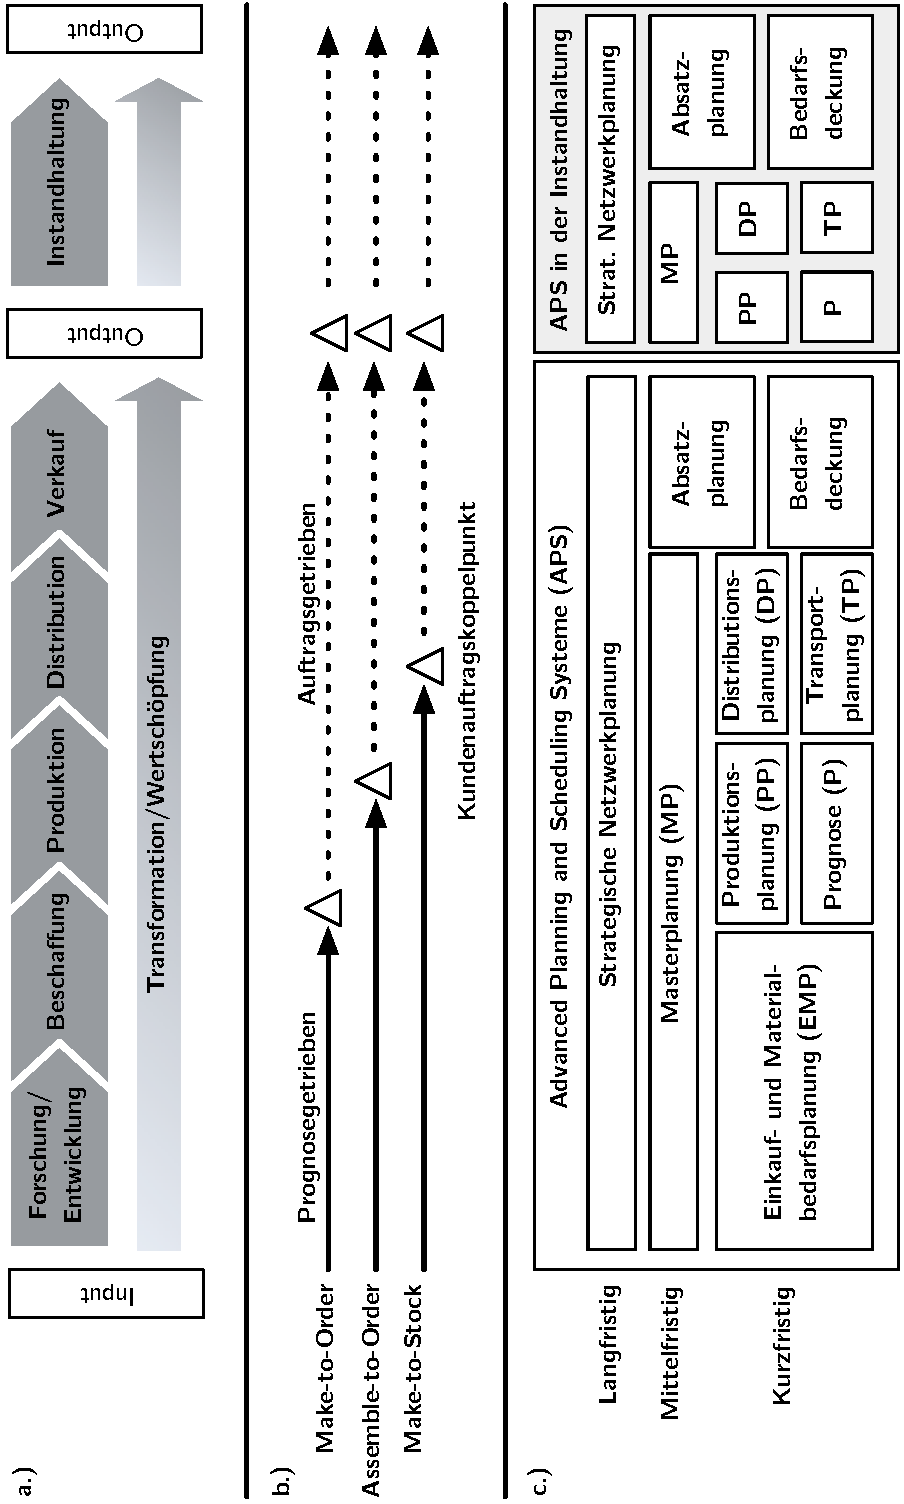
\includegraphics[width=120mm]{Bilder/prozess.pdf}
    \caption{Grafische Veranschaulichung eines Wertschöpfungsprozesses, der möglichen Kundenauftragskoppelpunkte und Advanced Planning and Scheduling Systeme}  \label{Prozess}
    {\footnotesize \textbf{In Anlehnung an:} \cite{Bach:2012aa}, S. 4-5; \cite{quante2009management}, S. 21-22; \cite{meyr2015structure}, S. 100}
  \end{center}
\end{figure}

Sofern das Unternehmen eine \textbf{Instandhaltung} als Leistungen anbietet, wird die Abfolge des Wertschöpfungsprozesses um dieses Unternehmenssystem erweitert. Dabei handelt es sich bei dem System der Instandhaltung um eine wiederholende oder erneute Wertschöpfung, indem das Unternehmen das zu reparierende Gut durch die angebotene Leistung erneuert. Für den gewerblichen Verkauf von Gütern an Privatkunden können gesetzliche Regelungen bestehen, womit ein Unternehmen gezwungen ist das Unternehmenssystem der Instandhaltung in den Wertschöpfungsprozess aufzunehmen.\footnote{Vgl. die Richtlinie 1999/44/EG des Europäischen Parlaments und des Rates vom 25. Mai 1999.} Anderseits kann ein Unternehmen auch die Instandhaltung seiner eigenen Güter als eigenständig angebotene Leistung bereitstellen und damit den Gesamtertrag des Unternehmens erhöhen (Auftragsfertigung). Dieses wird oft von Unternehmen angeboten, die ihren Umsatz mit komplexen Produkten erzielen.\footnote{Vgl. } Komplexe Produkte zeichnen sich durch ihre hohe Anzahl an hochtechnologischen Komponenten aus, die erst durch den vollständigen und meist kostenintensiven Zusammenschluss eine individuelle Bedürfnisbefriedigung des Nachfragers ermöglichen.\footnote{Vgl. \cite{komplexe2009Schmidt}, S. 97.} In dieser Arbeit werden solche komplexen Produkte betrachtet, die aus einer Vielzahl von Komponenten bzw. Ressourcen bestehen. Dementsprechend handelt es sich bei den in dieser Arbeit betrachteten Instandhaltern um Anbieter von komplexen Produkten. 

Weiter versteht \citeauthor{helbing2010instandhaltung} unter Instandhaltung die \glqq Gesamtheit der technischen und organisatorischen Mittel, Vorgänge und Maßnahmen zur Erhaltung, Verbesserung und Wiederherstellung des Funktions-, Leistungs- und Güteniveaus von materiellen Objekten während ihrer Wirkungs- und Lebenszeit durch Wartung, Inspektion und Instandsetzung.\grqq\footnote{Vgl. \citeauthor{helbing2010instandhaltung}, S. 984} In dieser Arbeit ist unter dem Begriff der Instandhaltungsprozesse gemeint, dass für den Reparaturauftrag des betrachteten komplexen Produkts ein spezifischer Ausführungsmodus verwendet werden kann, der eine erneute Integration von produkt-spezifischen Ressourcen vorsieht, damit die Funktionsfähigkeit des Produkts wiederhergestellt ist. Damit lässt sich das Verständnis des Begriffs als Leistung eines Unternehmens und als Unternehmenssystem ableiten, welches die Verlängerung und zugleich die Erweiterung des Wertschöpfungsprozesses versteht. Abbildung \ref{Prozess} zeigt im Teil a den erweiterten Wertschöpüfungsprozess eines produzierenden Unternehmens inkl. der Integration des Teilsystems der Instandhaltung.

\section{Charakteristika}

Nach der DIN 310511 wird Instandhaltung insofern ausgeführt, wenn die Funktionsfähigkeit einer Betrachtungseinheit sichergestellt werden muss, damit der ursprüngliche Wert erhalten bleibt.\footnote{Vgl. \cite{Strunz:2012aa}, S. 1.} Betrachtungseinheit können ganze Anlagen und Maschinen sein oder nur einzelne Komponenten.\footnote{Vgl. \cite{schenk2010techSys}, S. 23.}

Erläuterung nach DIN 31051:\footnote{Unbedingt nachlesen!!!!}
\begin{itemize}
\item Instandhaltung ist die Kombination aller technischen und administrativen Maßnahmen des Managements während des Lebenszyklus einer Betrachtungseinheit zur Erhaltung des funktionsfähigen Zustandes oder der Rückführung in diesen, so dass sie die geforderte Funktion erfüllen kann.
\item Als Betrachtungseinheit (BE) wird jedes Bauelement, Gerät, Teilsystem, jede Funktionseinheit, jedes Betriebsmittel oder System, das für sich allein betrachtet werden kann, definiert.
\end{itemize}

Nach der DIN 31051 werden Einheiten betrachtet, die eine Wartung, Inspektion, Instandsetzung oder Verbesserung bedürfen.\footnote{Vgl. \cite{schenk2010techSys}, S. 23-24.} Bei einer Wartung handelt es sich um Maßnahmen zur Verzögerung der Abnutzung. Die Inspektion umfasst alle Maßnahmen der Begutachtung sowie der Beurteilung des Ist-Zustandes einer Betrachtungseinheit und die Instandsetzung beinhaltet die Maßnahmen zur Wiederherstellung des Sollzustands. Mit der Verbesserung sind Maßnahmen gemeint, die den Soll-Zustand der Betrachtungseinheit erweitern, damit mögliche Defekte verhindert werden. In dieser Arbeit wird bei auftragsbezogenen Instandhaltungsprozessen nur die Instandsetzung von Produkten betrachtet.

Instandhaltungsprozesse lassen sich weiter nach Ausführungszeitpunkt und Ausführungsort der Maßnahmen unterscheiden.\footnote{Vgl. \cite{schenk2010techSys}, S. 24-26; \cite{hinsch2010instandhaltung}, S. 190-191.} Diese Unterscheidung spielt bei der Betrachtung von auftragsbezogenen Instandhaltungsprozessen eine untergeordnete Rolle und wird daher im Verlauf der Arbeit nicht mehr betrachtet.

Da der Absatz zeitlich vor der Produktion der Leistung stattfindet, handelt es sich bei den hier betrachteten auftragsbezogenen Instanhaltungsprozessen um eine Auftragsfertigung.\footnote{Vgl. \cite{hax1956industriebetrieb}, S. 247; \cite{Gutenberg1965dispos}, S. 164-165.} In der wissenschaftlichen Literatur wird für die Auftragsfertigung oft der englischen Begriff \textit{Make-to-Order} verwendet (Abk. MTO). Abzugrenzen ist der Begriff von der Lagerfertigung (engl. Make-to-Stock; Abk. MTS) und der kundenindividuellen Fertigung mit standardisierten Komponenten (engl. Assemble-to-Order, Abk. ATO). 
Eine Abgrenzung kann zum einen anhand des Kundenauftragskoppelpunkts und zum anderen anhand der Planungsgrundlage der Leistungserstellung getätigt werden.\footnote{Vgl. ???} Der Kundenauftragskoppelpunkt zeigt den erstmaligen Kundenkontakt bzw. Auftragseingang auf.\footnote{Vgl. ???} Mit Eingang des Kundenauftrags wechselt die Planungsgrundlage der Leistungserstellung von prognosegetriebener hin zu auftragsgetriebener Planung. Die prognosegetriebene Planungsgrundlage für die Fertigung ist mit einem Prognosefehler für die Ausführung der unternehmerischen Tätigkeit behaftet, was der Betrachtung des Kundenauftragskoppelpunkts zur Bestimmung der notwendigen Ressourcenkapazität und der weiteren Auftragseingänge weiteres Gewicht verleiht.\footnote{Vgl. \cite{quante2009management}, S. 21.} 

Bei einem MTO-Auftrag trifft vor der eigentlichen Produktion der Leistung der Kundenauftrag ein. D. h. das Unternehmen startet erst nach Annahme des Auftrags mit der Leistungserstellung. Damit sind die Forschungs/Entwicklung der Leistung und die Beschaffung der Komponenten bzw. der Ressourcen hauptsächlich prognosegetrieben. Alle weiteren Teilsysteme des Unternehmens können sich speziell an den Forderungen des Auftrags richten. Ähnliche Rahmenbedingung besitzt eine ATO, die den Kundenauftragskoppelpunkt innerhalb des Produktionsablaufs hat. Da nur ein gewissen Umfang der Komponenten an auftragsspezifischen Eigenschaften angepasst wird, sind die Grundkomponenten der Produkte abhängig der Prognosen des Unternehmens über einen möglichen Absatzverlauf. Bei MTS erfolgt der Auftragseingang erst nach der Produktion, womit diese Fertigungsart den höchsten Anteil des Einsatzes von betrieblicher Prognosemethoden aufweist, damit ein ausreichendes Absatzvolumen produziert wird.\footnote{Vgl. \cite{fleischmeyr2004codp}, S. 300-303; \cite{quante2009management}, S. 21-22} Abbildung \ref{Prozess} zeigt im Teil b die Unterschiede der Fertigungsarten im Verlauf des Wertschöpfungsprozesses. 

Da bei auftragsbezogenen Instandhaltungsprozessen erst mit Auftragseingang die erforderlichen Produktionsschritte und der Ressourcenbedarf bekannt sind, werden diese mit MTO-Prozessen gleichgesetzt. Zur Erfüllung möglichst vieler Aufträge muss eine möglichst gute Prognose der benötigen Ressourcen vorliegen, damit kurze Liefer- und Durchlaufzeiten gewährleistet bleiben.\footnote{Vgl. \cite{thaler2001supply}, S. 68.} Sofern die Prognose fehlerhaft ist und damit ein zu geringer Bestand an Ressourcen vorhanden ist, konkurrieren die unterschiedlich eintreffenden Anfragen nach der Instandsetzungsleistung des Unternehmens bzgl. der Ressourcen untereinander. Sofern ein zu hoher Ressourcenbestand vorhanden ist, stellt sich die Frage über den besten Mix der unterschiedlichen Aufträge, damit die Ressourcenkapazität optimal genutzt wird und dementsprechend der Ertrag maximiert wird. Unrentable Anfragen sollten abgelehnt werden, damit die dadurch nicht verbrauchten Ressourcen für spätere rentablere Anfragen Verwendung finden. Im nächsten Abschnitt wird dieser Frage in Bezug von Produktionsplanungssystemen und der betrieblichen Entscheidungsfindung weiter nachgegangen.


\section{Relevanz für betriebliche Entscheidungen}

Die Entscheidungen über die mögliche Ausgestaltung der Politik über die Annahme oder die Ablehnung der eingehenden Kundenaufträge besitzt einen großen Einfluss auf den Gesamtertrag und auf die Effizienz des gesamten SCM-Prozesses eines Unternehmens.\footnote{Vgl. } Ein effizienter SCM-Prozess kann der nachhaltigen Konsumentenzufriedenheit dienen.\footnote{Vgl. } Wichtiger Erfolgsfaktor für ein erfolgreiches SCM und somit der Konsumentenzufriedenheit ist der Einsatz von Advanced Planning and Scheduling Systemen (APS).\footnote{Vgl. \cite{fleischmeyr2004codp}, S. 298}

Bei APS handelt es sich um computergestützte Systeme, mit denen die Planung der ganzheitlichen Wertschöpfung der Leistung mit Hilfe von mathematischer Modelle des Operations Research unterstützt wird.\footnote{Vgl. \cite{fleischmeyr2004codp}, S. 298. \label{fleisch}} Neben der reinen Planung der Produktion, helfen moderne APS mit ihrem modularen Aufbau auch bei der gesamten Auftragsabwicklung und unterstützen damit Unternehmen bei betrieblichen Entscheidungen innerhalb des SCM-Prozesses, wie z. B. bei dem Einkauf von Ressourcen, der Produktionsplanung und dem Absatz der Leistung.\footnote{Vgl. \cite{meyr2015structure}, S. 99-100; \cite{fleischmeyr2004codp}, S. 298.}

\cite{meyr2015structure} sortieren einige wichtige Module eines APS in den Dimensionen des SCM-Prozesses und des Planungshorizonts. Abbildung \ref{Prozess} in Teil c greift diese Sortierung auf. Bei dem Modul der strategischen Netzwerkplanung werden die Lieferanten, Werke und Lagerpunkte in einer langfristigen Betrachtungsweise festgelegt. Die Entscheidungen die Aufgrund der strategischen Netzwerkplanung getroffen werden, haben erheblichen Einfluss auf die langfristige Rentabilität sowie Wettbewerbsposition des Unternehmens und haben räumlichen sowie zeitlichen Charakter.\footnote{Vgl. \cite{goetschalckx2005strategic}, S. 117-118.} Typische Entscheidungen die aufgrund des Moduls der strategischen Netzwerkplanung getroffen werden, sind die Festlegungen des Kunden- und Produktprofils des Unternehmens über einen längeren Betrachtungszeitraum. Aber auch grundlegende Entscheidung bzgl. des Herstellungsprozesses des Unternehmens werden aufgrund dessen abgeleitet. Datengrundlage für diese Planung bilden u. a. Prognosen, Marktforschungen und Wirtschaftstrends.
Die Absatzplanung dient einerseits der Absatzprognose und anderseits der Analyse der notwendigen Sicherheitsbestände.\footref{fleisch} Das Modul Masterplanung synchronisiert den Materialfluss entlang des gesamten SCM-Prozesses und unterstützt dadurch mittelfristige Entscheidungen über die effiziente Nutzung der Ressourcen, damit für einen kontinuierlichen Materialfluss größere Puffer gemieden werden.\footnote{Vgl. \cite{rohde2002scm}, S. 143.} Mit dem Modul der Einkaufs- und Materialbedarfsplanung werden kurzfristig terminierte Pläne für Komponenten und Teile (Ressourcen) für die Fertigung berechnet.\footnote{Vgl. \cite{stadler2008aps}, S. 217-218.} Aufbauend auf diesen Plänen kann die Produktionsplanung und die weitere Prognose für die Produktion und Logistik erfolgen, die den organisatorischen Anforderungen des Produktionssystems gerecht werden müssen und einen kurzfristigen Planungshorizont aufweisen.\footref{fleisch} Bei diesen Modulen werden in einer kurzfristigen Betrachtung u. a. die Maschinenverfügbarkeit und die Losgrößen geplant bzw. prognostiziert. Eine effiziente Produktionsplanung setzt eine gute Prognose voraus.\footnote{Vgl. \cite{dickersback2004pp}, S. 131.} Bei den Modulen der Distributions- und Transportplanungen werden Pläne für die Verkaufsstellen und für die Logistik generiert.\footref{fleisch} Zum Abschluss wird das Modul Available-to-promise (ATP) aufgeführt. Bei ATP handelt es sich um ein System, mit dem Kundenaufträge auf Realisierbarkeit in Bezug der aktuellen und zukünftigen Verfügbarkeit von Angebot und Kapazität analysiert werden.\footnote{Vgl. \cite{Stadtler:2008aa}, S. 183.} Das Modul dient hauptsächlich der Kundenzufriedenheit, da es die eintreffenden Kundenaufträge prüft und ggf. die geforderte Lieferung der Leistung zusagt.\footref{fleisch}

Die vorgestellten Module sind von \cite{meyr2015structure} jedoch im Verhältnis eines typischen SCM-Prozess gesetzt. Es stellt sich die Frage, welche Systeme für betriebliche Entscheidungen durch Einbeziehung eines Instandhaltungsprozesses in den SCM-Prozess relevant sind. Die Instandhaltung verlängert den Wertschöpfungsprozess des Unternehmens und benötigt den Einsatz von speziellen APS-Systemen. Jedoch kann eine Teilmenge der Systeme nach \cite{meyr2015structure} auch auf Instandhaltungsprozesse übertragen werden, da diese der Auftragsfertigung gleichgesetzt werden können. Es handelt sich um die Systeme die sich aufgrund der Produktion einer Leistung ergeben, aber auch um ein System in Anlehnung an das System ATP. Ebenfalls bedarf es langfristiger Entscheidungsunterstützung in Bezug der strategischen Netzwerkplanung. Mit dem Modell lässt sich ableiten, welche Ausgestaltung die Leistung der Instandhaltung erhält. Die Masterplanung, die für mittelfristige Entscheidung notwendig ist, unterstützt den Ressourceneinsatz über einen gewissen vordefinierten Planungshorizont und ist damit ebenfalls für die mögliche Ressourcenverwendung bei Instandhaltungsaufträgen von Nöten. Für systemgestützte Entscheidungen zur Instandhaltung bedarf es für die kurzfristiger Betrachtungsweise an Input der Einkaufs- und Materialplanung. Bei diesen Informationen kann es z. B. um den aktuellen Lagerbestand oder den Zeitpunkt von Lieferung neuer Produktionsrohstoffe handelt. Bei auftragsbezogenen Instandhaltungsprozessen wird unterstellt, dass eine Entscheidung bzgl. der Auftragsannahme auf Basis des Systems ATP im Vorfeld getätigt werden muss. D. h. die Entscheidungsgrundlage über die Annahme oder Ablehnung eines Auftrags muss im Vorfeld der Produktionsplanung vorliegen. Ebenso sind Prognosen über mögliche weitere Auftragseingänge zur diesem Zeitpunkt und für die nachfolgenden Entscheidungen zu beachten. Erst mit Informationen über den aktuellen Bestand an Ressourcen sowie seinen möglichen Verlauf und einer Prognose über die weitere Auftragsentwicklung  ist die Annahme und damit eine Beachtung des Auftrags in der Produktions- und Transportplanung möglich.

Für auftragsbezogene Instandhaltungsprozesse bedarf es daher einer speziellen Masterplanung in Form einer optimalen Politik der effizienten Nutzung der Ressourcen. Ein Unternehmen benötigt für die kurzfristige Entscheidung der Annahme oder Ablehnung von Instandhaltungsaufträgen Informationen eines umfangreichen Masterplans mit langfristigen Planungshorizont. Dabei kann für die Erstellung einer solchen Masterplanung für MTO- bzw. auftragsbezogene Instandhaltungsprozesse anhand des Konzepts des Revenue Managements erfolgen. Dabei liefert eine solche Planungsgrundlage für jede noch verfügbare Ressourcenkapazität und für jeden Zeitpunkt des Planungshorizonts eine optimale Politik der Akzeptanz von Aufträgen. Diese Planung erfolgt unter Beachtung des angebotenen Leistungsprogramms und einer Prognose über den möglichen weiteren Auftragsverlauf. Im weiteren Verlauf dieser Arbeit wird das Grundmodell des Revenue Managements vorgestellt (Kapitel \ref{KapitelDP}) und ein Modell speziell für auftragsbezogenen Instandhaltungsprozesse aufgestellt (Kapitel \ref{HauptteilDP}). Mit einem Masterplan aufgrund des Modells des Revenue Managements ist eine verbesserte Kapazitätsauslastung für das Unternehmen möglich.\footnote{Vgl. }





